\documentclass[conference]{IEEEtran}

\usepackage[T1]{fontenc}
\usepackage{amsmath,amssymb}
\usepackage{booktabs}
\usepackage{array}
\usepackage{enumitem}
\usepackage{cite}
\usepackage{tikz}
\usetikzlibrary{arrows.meta,positioning,fit,backgrounds,calc,patterns}
\usepackage[hidelinks]{hyperref}
\newcommand{\doi}[1]{doi:\,\url{#1}}

\setlist{itemsep=1pt,topsep=2pt,leftmargin=*}
\newcommand{\todo}[1]{\textcolor{red!70!black}{[#1]}}
\usepackage{xcolor}
\usepackage{algorithm}
\usepackage{algpseudocode}

\begin{document}

\title{Change-Characteristic-Aware Window Selection for Unsupervised Concept Drift Detection in Real-Time Text Streams}

\makeatletter
\newcommand{\linebreakand}{\end{@IEEEauthorhalign}\hfill\mbox{}\par\mbox{}\hfill\begin{@IEEEauthorhalign}}
\makeatother

% \author{
% \IEEEauthorblockN{Md. Abu Towsif}
% \IEEEauthorblockA{26-93964-1@student.aiub.edu\\
% American International\\University-Bangladesh}
% \and
% \IEEEauthorblockN{Farjana Yesmin Opi}
% \IEEEauthorblockA{{26-93965-1@student.aiub.edu}\\
% American International\\University-Bangladesh}
% \and
% \IEEEauthorblockN{Mst. Nadiya Noor}
% \IEEEauthorblockA{{26-94277-3@student.aiub.edu}\\
% American International\\University-Bangladesh}
% \linebreakand
% \IEEEauthorblockN{Md. Jahid Hasan}
% \IEEEauthorblockA{{26-94240-@student.aiub.edu}\\
% American International\\University-Bangladesh}
% \and
% \IEEEauthorblockN{Hasibur Rashid Chayon}
% \IEEEauthorblockA{{chayon@aiub.edu}\\
% American International\\University-Bangladesh}
% }

\maketitle

%--------------------------------------------------------------------
\section{Introduction}

Text is produced continuously by news feeds, review sites and social platforms. Their topics and vocabulary change over time and a model trained on older documents slowly becomes outdated. For example a news classifier encounters new subjects and terms after a major event. This change in the data-generating process is called concept drift \cite{gama2014,lu2019} (Fig.~\ref{fig:drift}). Real-time systems must notice it because the usual remedy is to update the model on recent data which costs computation and often new annotations. Text streams also show three characteristics of big data. They have high velocity as documents arrive continuously and must be processed in a single pass. They have variety because the documents are unstructured and differ in topic, source and style. And their veracity is uncertain since labels are missing and the true drift points are usually unknown.


For text, the problem is harder because labels arrive late or never \cite{garcia2024review}. Classic detectors watch a classifier's error rate and need the true label after every prediction \cite{gama2004,bifet2007} so a text detector has to work without labels. It should identify a genuine change quickly while avoiding alarms caused by ordinary fluctuations. A late alarm keeps an outdated model in use whereas a false alarm can trigger an unnecessary update and may need additional labeling costs. Lukats et al.\ \cite{lukats2025} showed that accuracy-based scores can favor detectors that fire often, highlighting the need to evaluate detection delay and false alarms separately.

\begin{figure}[!t]
\centering
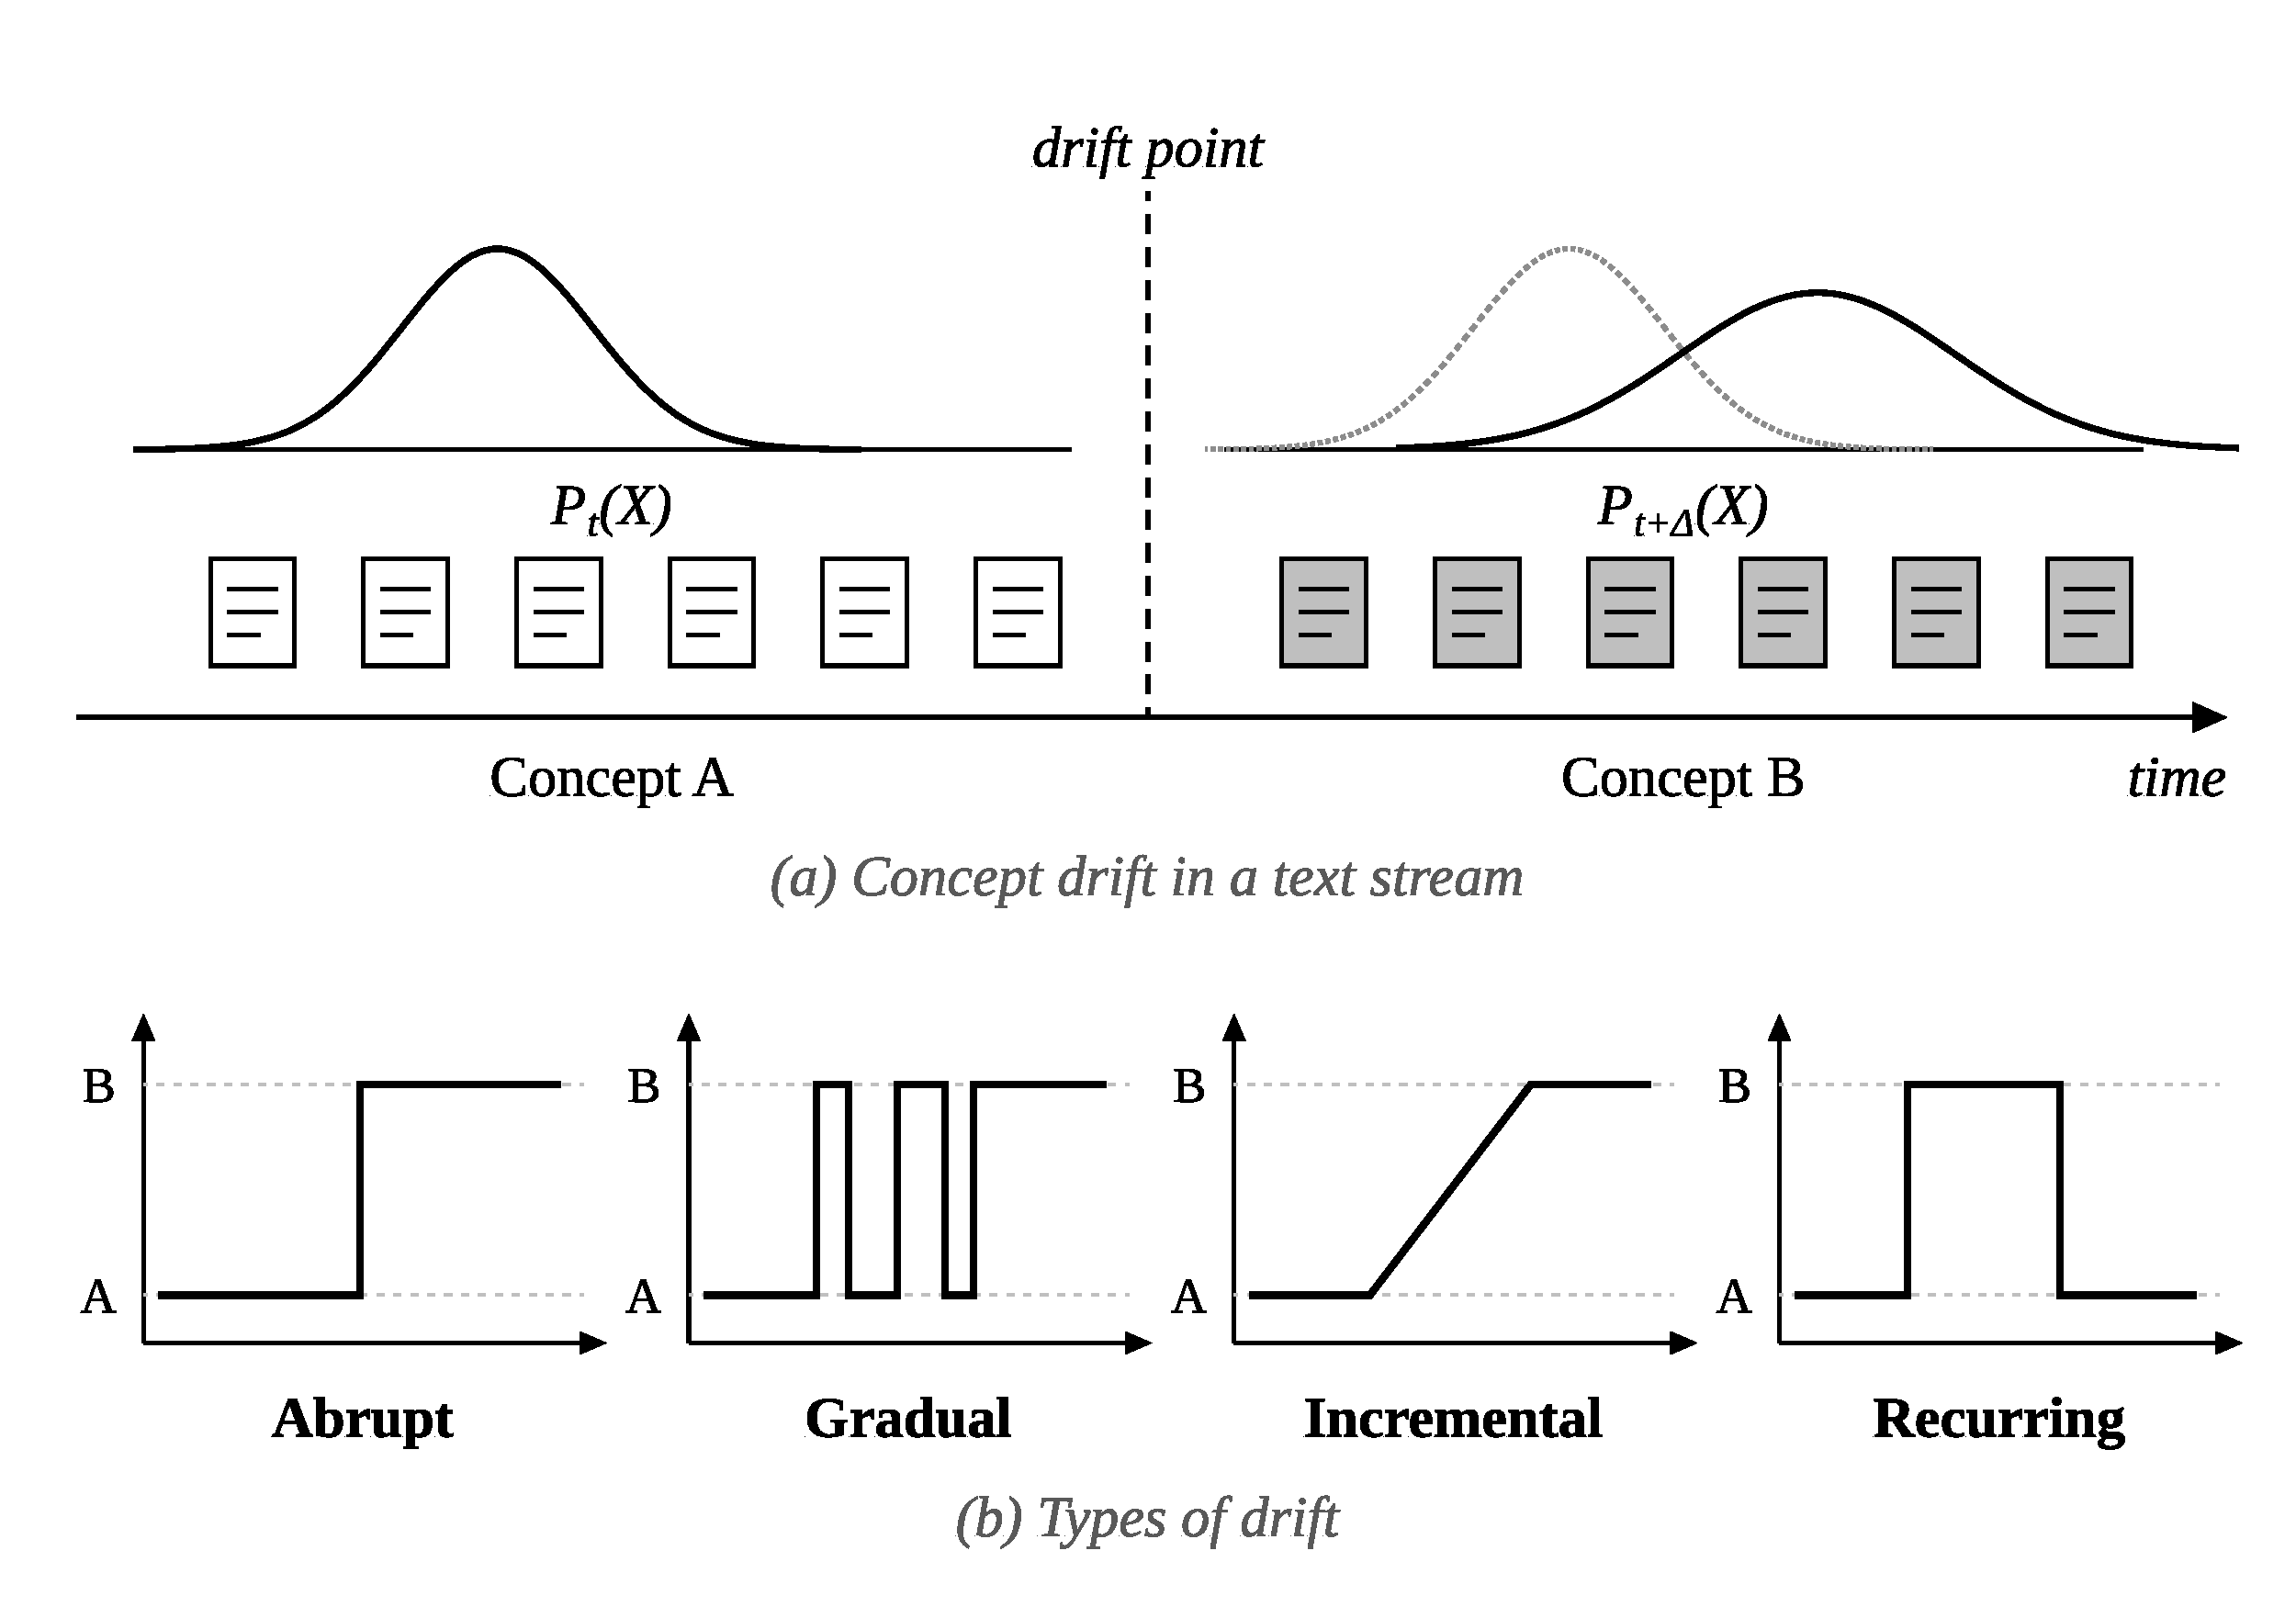
\includegraphics[width=\linewidth]{figures/concept_drift.pdf}
\caption{Concept drift. (a) The distribution of incoming documents changes from $P_t(X)$ to $P_{t+\Delta}(X)$ at the drift point; the dotted curve shows the old distribution. (b) Common drift types by how the concept changes over time.}
\label{fig:drift}
\end{figure}



Unsupervised detectors usually compare a window of recent data with a window of older data \cite{hinder2024a}. A short window reacts fast but is sensitive to noise while a long window is stable but slow. The best size also depends on the drift since a gradual or subtle change needs more data to stand out than an abrupt one. The benchmark in \cite{lukats2025} names better window-size selection as open future work.
ADWIN \cite{bifet2007} avoids a fixed size by keeping a variable-length window and cutting it when two parts differ according to a Hoeffding-type bound. It is mostly applied to classifier errors which needs labels. ADWIN-U \cite{assis2025} removes this need by monitoring simple statistics of each example such as skewness and kurtosis which worked best in its tests on ten numeric streams. It is our starting point. Three issues still need to be addressed. These include its fixed confidence level $\delta$, dropping the whole older sub-window after each detection whatever the strength or persistence of the change and evaluation only on numeric sensor-type streams. For text it is not clear whether these statistics can detect topic changes in sentence embeddings.

We study a window-selection policy built on ADWIN-U. At first, the detector looks at how strong and how persistent the unlabeled evidence is and then chooses between a full cut, a hold and a partial cut of the window. It reuses ADWIN's bucketed window so its cost per instance should stay close to that of ADWIN-U. In terms of these characteristics, the policy handles velocity with a compact window that is updated in constant time, variety by working on sentence embeddings of unstructured text and veracity by using no labels and by not acting on a single weak signal. Our work check whether this improves the balance between delay, false alarms and missed drift on text streams and how the effect depends on drift type and magnitude. We also measure how much time and memory it uses and check whether the results from added drift also apply to a real stream where the drift points are unknown.

The main contributions of our work are:
(i) We propose a label-free window-selection policy with a hold state and a graded cut that contains ADWIN-U as a special case at the same $O(\log W)$ cost.
(ii) We show that graded cutting lowers detection delay on gradual and subtle drift at a matched false-alarm rate, while abrupt drift is handled as in ADWIN-U.
(iii) We examine whether ADWIN-U's per-instance statistics capture topic drift in sentence embeddings, compared with a centroid-distance signal.


Our contribution is not the adaptive window or the label-free monitoring itself which ADWIN and ADWIN-U already provide. It is the rule that decides how the window changes after evidence of drift and its evaluation on text.

The rest of the paper is organized as follows. Section~\ref{sec:related} covers related work and Section~\ref{sec:method} explains the proposed method and Section~\ref{sec:exp} describes how we plan to evaluate it.

%--------------------------------------------------------------------
\section{Background and Related Work}
\label{sec:related}

\subsection{Concept drift and its types}

A data stream is a sequence of instances arriving over time. Concept drift occurs between times $t$ and $t+\Delta$ if the joint distribution changes, $P_t(X,Y)\neq P_{t+\Delta}(X,Y)$ \cite{gama2014}. Changes in $P(X)$ alone are called virtual drift or feature change. Detectors that use no labels can only observe this kind \cite{assis2025}. Drift is commonly grouped by its speed and shape into abrupt, gradual, incremental and recurring drift \cite{webb2016,suarez2023}. Abrupt drift replaces one concept by another at a single point. Gradual drift mixes the old and new concept for a period. Recurring drift occurs when a previously seen concept returns such as with seasonal changes. Reviews of the field \cite{gama2014,lu2019} also cover how models are adapted after a detection.

\subsection{Supervised and unsupervised detectors}

Supervised detectors such as DDM \cite{gama2004} and ADWIN \cite{bifet2007} watch the error of a classifier and need the true label soon after each prediction. Assis and Souza note that this is unrealistic in many applications and that unsupervised methods are still a small part of the literature \cite{assis2025}.

Unsupervised detectors compare the distribution of recent and older data. Hinder et al. describe this as a common approach where two windows are selected and each is summarized before testing a dissimilarity score \cite{hinder2024a}. They also list how the reference window can be kept and most approaches use sliding windows. For example, KSWIN which applies the Kolmogorov--Smirnov test inside a sliding window \cite{raab2020} and D3 which trains a classifier to separate old from new instances and watches its AUC \cite{gozuacik2019}. Lukats et al.\ \cite{lukats2025} surveyed ten fully unsupervised detectors and compared seven on eleven real-world streams. No detector won on every metric and classifier accuracy can favor detectors that fire often since frequent updates keep the model fresh. For this reason we report delay and false alarms directly and we use accuracy-based scores only as secondary evidence. The same study suggests automatic selection of window sizes as future work.

\subsection{Adaptive windows}

ADWIN \cite{bifet2007} maintains a window $W$ and examines every split $W=W_1\cdot W_2$. A change is declared when $|\hat\mu_{W_1}-\hat\mu_{W_2}|\ge\varepsilon_{\mathrm{cut}}$ where the bound $\varepsilon_{\mathrm{cut}}$ comes from Hoeffding's inequality \cite{hoeffding1963} and depends on a confidence level $\delta$. Once a change is detected, the older part $W_1$ is dropped. To stay cheap, ADWIN stores the window as an exponential histogram \cite{datar2002} which requires $O(\log W)$ memory and time.

Several other methods follow different strategies for adjusting the window. DAWIDD, for instance, examines the statistical dependence between the observed data and time to determine whether a change has occurred \cite{hinder2020}. Chen et al.\ use a short and a long variable window with a decay model to separate drift types in frequent pattern mining \cite{chen2024}. Klinkenberg and Joachims \cite{klinkenberg2000} and Kuncheva and \v{Z}liobait\.{e} \cite{kuncheva2009} choose the window size from estimated classification error or from theory so they need labels or a classifier. Window handling also appears in applied systems. Mehmood et al.\ combine an LSTM with the Page--Hinkley test, ADWIN and KSWIN for sensor forecasting on an edge architecture \cite{mehmood2024}. Badar et al.\ use EDDM to update a sliding window in federated stream classification \cite{badar2023}. Hu et al.\ adjust a model's enclosing ball by expanding and contracting it so that it follows new concepts without growing too large \cite{hu2024}. These works adjust windows or models in several ways but none of the studies we reviewed defines a general label-free policy for deciding how much of a window to drop.

\subsection{ADWIN-U}

ADWIN-U \cite{assis2025} keeps the ADWIN windowing and replaces the monitored value. From each example it extracts a descriptive statistic $s_i$ (for example skewness or kurtosis over the feature values) and feeds it to ADWIN. It has a single-detector form with one window and a multiple-detector form with one window per predicted class where an alarm in any window restarts all of them. In the authors' tests on ten real numeric streams, skewness and kurtosis worked best with multiple detectors and the geometric mean worked best with a single detector. The cost stays at $O(\log W)$ per instance for one detector and $O(l\log W)$ for $l$ detectors. The authors also propose the BAR score which combines accuracy with the share of labels requested for model updates. They set $\delta=0.002$ in their experiments and suggest monitoring several statistics at once through voting or dynamic selection as future work.

\subsection{Text streams}

Garcia et al.\ reviewed drift adaptation in text stream mining and point out that few text benchmarks come with labeled drift points \cite{garcia2024review}. Text is turned into vectors with pre-trained encoders such as Sentence-BERT \cite{reimers2019}. Whether the simple statistics that work for numeric sensor data also react to topic drift in embeddings has not been tested. To our knowledge, ADWIN-U-style windowing has not been evaluated on text streams although a systematic literature search is still needed to confirm this.

In summary, window choice shapes what a detector sees, ADWIN-U provides a label-free adaptive window and text streams lack a tested evaluation protocol. What is still missing is a rule that uses the strength and persistence of unlabeled evidence to decide how the window changes and an evaluation of that rule on text.

\begin{figure*}[!t]
\centering
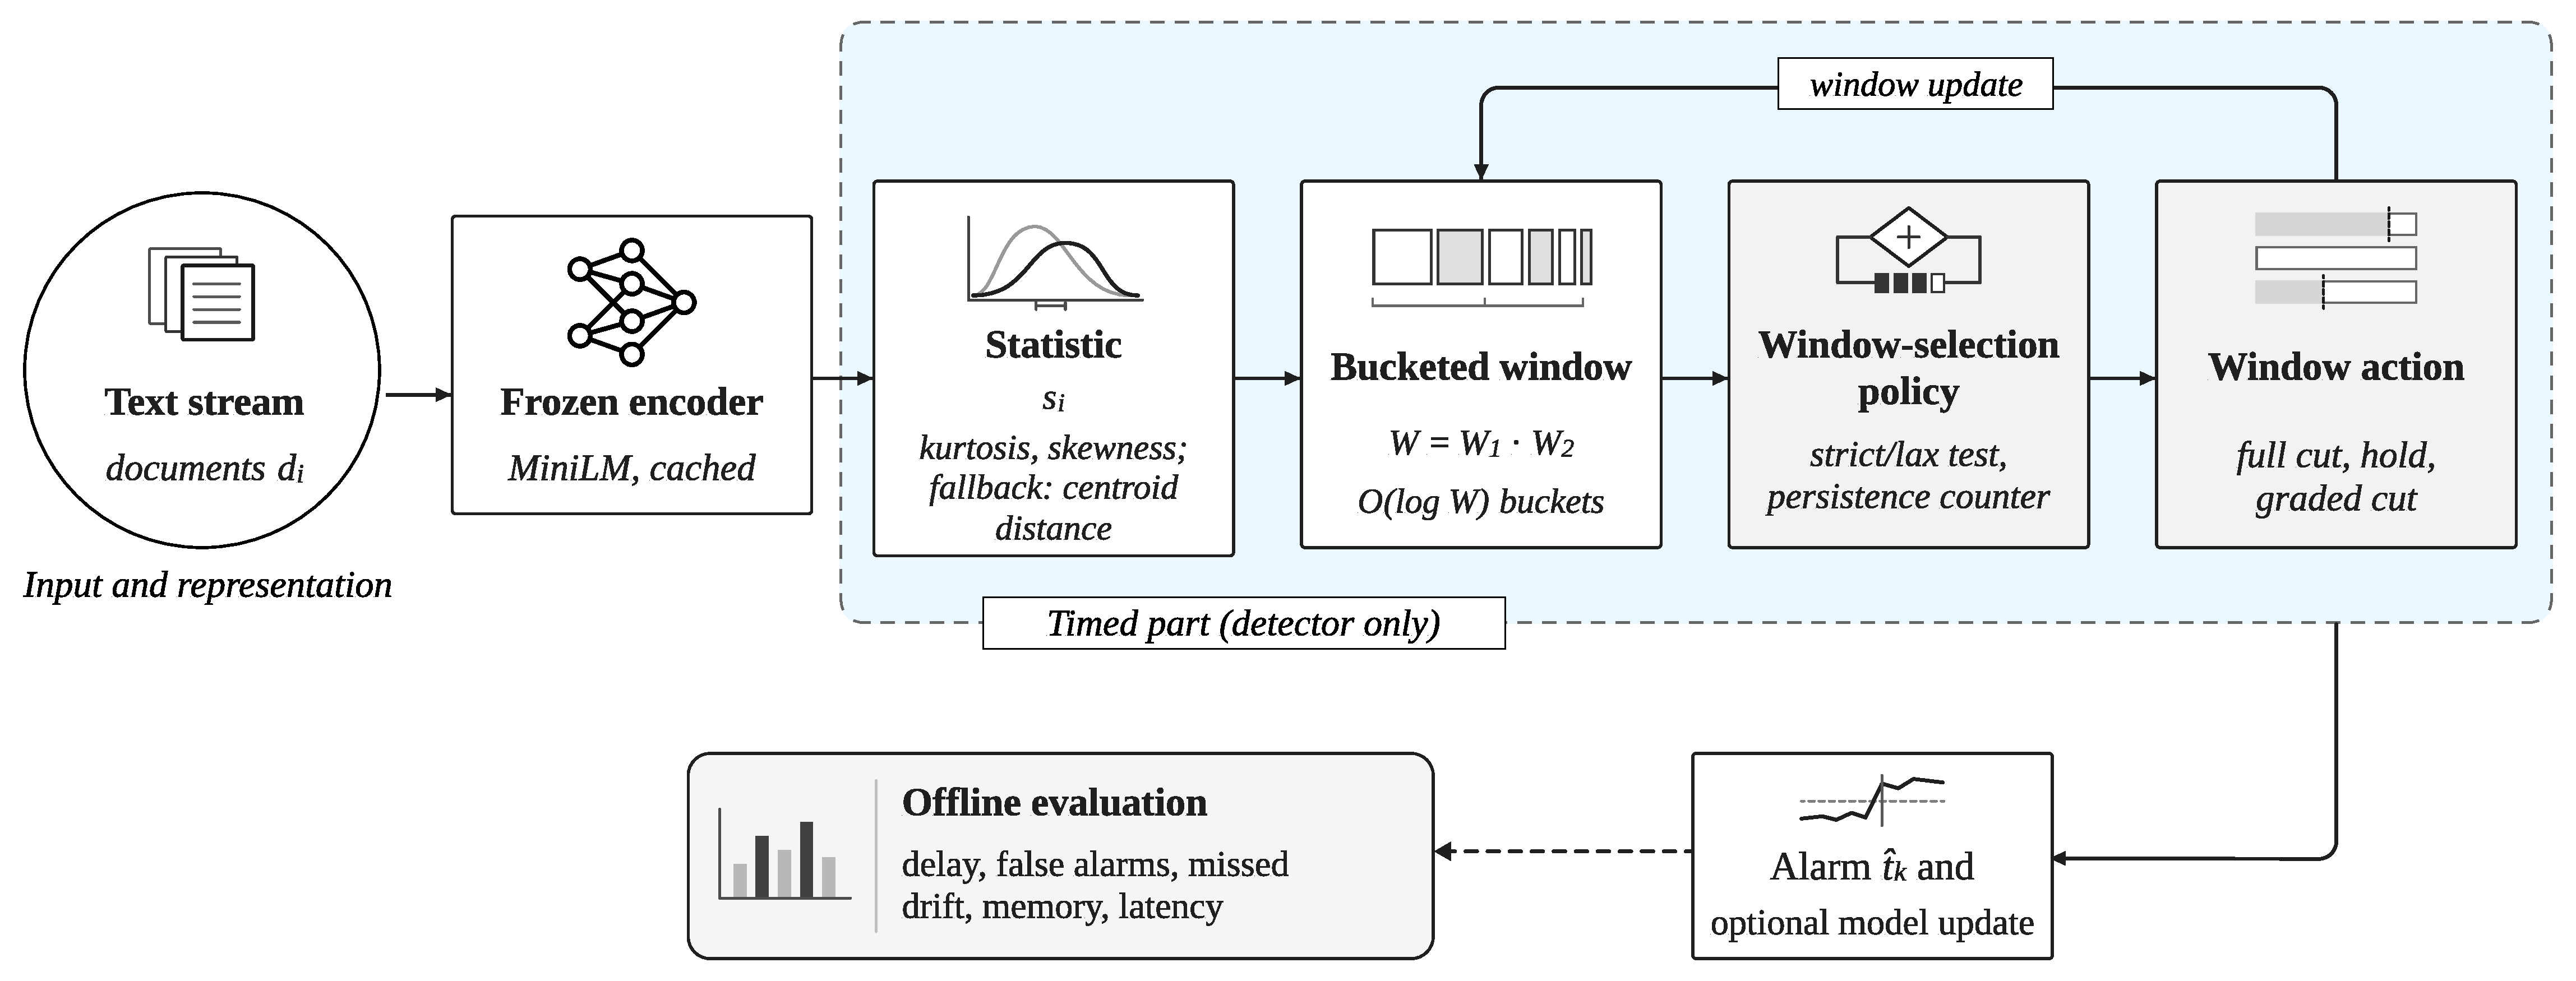
\includegraphics[width=\linewidth]{figures/pipeline.pdf}
\caption{Overview of the proposed framework. Embeddings are computed once and cached, so the timed part covers only the detector. Shaded boxes mark the new component.}
\label{fig:pipeline}
\end{figure*}

\section{Methodology}
\label{sec:method}

This section first defines the problem and gives an overview of the framework. It then describes each stage of the detector and its cost.

\subsection{Problem formulation}
\label{sec:problem}

A text stream is an unbounded sequence of documents $S=(d_1,d_2,\dots)$ that arrive one at a time. A frozen encoder $f$ maps each document to an embedding $x_i=f(d_i)\in\mathbb{R}^D$. The stream contains an unknown set of drift points $\mathcal{T}=\{t_1,t_2,\dots\}$ at which the distribution of $x_i$ changes. The detector reads each $x_i$ once, never sees a label, keeps only a compact summary of the past and outputs a set of alarm times $\hat{\mathcal{T}}=\{\hat t_1,\hat t_2,\dots\}$. Labels are used only to build streams with known drift and to train an optional downstream classifier.

A good detector raises an alarm soon after each $t_m\in\mathcal{T}$, raises few alarms when nothing changes and misses no drift. It must also keep its time and memory per document small enough to keep up with the stream. Section~\ref{sec:metrics} turns these goals into measurable quantities.

\subsection{Framework overview}

Fig.~\ref{fig:pipeline} shows the framework. It has four stages. (1) Each document is encoded once and the embedding is cached. (2) A scalar drift signal $s_i$ is computed from the embedding. (3) The signal is inserted into an adaptive window that is stored as buckets, as in ADWIN. (4) At each check, the window-selection policy reads the evidence in the window and decides whether to keep, partly cut or fully cut it. Stages 2 to 4 form the detector and are the only part we time. Stages 2 and 3 follow ADWIN-U, and stage 4 is our contribution.

\subsection{Text representation and drift signal}

\subsubsection{Encoder}
Documents are encoded with the Sentence-BERT model \texttt{all-MiniLM-L6-v2} \cite{reimers2019}, which is distilled from MiniLM \cite{wang2020} and produces $D=384$ dimensional vectors. The encoder is not fine-tuned, so the representation itself does not drift. Caching the vectors keeps encoding time out of the detector timings.

\subsubsection{Per-instance statistic}
Following ADWIN-U \cite{assis2025}, we reduce each embedding to one number computed over its $D$ components. With $\bar x_i$ and $\sigma_i$ the mean and standard deviation of the components of $x_i$, the kurtosis and skewness signals are the sample moments used in ADWIN-U \cite{assis2025,joanes1998}:
\begin{equation}
s_i^{\mathrm{kurt}}=\frac{1}{D}\sum_{j=1}^{D}z_{ij}^{4},\quad
s_i^{\mathrm{skew}}=\frac{1}{D}\sum_{j=1}^{D}z_{ij}^{3},\quad
z_{ij}=\frac{x_{ij}-\bar x_i}{\sigma_i}.
\label{eq:stat}
\end{equation}
These statistics worked best with multiple detectors on numeric streams in \cite{assis2025}, but a change of topic may leave the shape of an embedding's components unchanged. We therefore test them first and compare them with the centroid signal (Section~\ref{sec:exp}).

\subsubsection{Centroid-distance signal}
As a backup signal that is closer to the meaning of the text, we use the cosine distance \cite{salton1975} between $x_i$ and a running centroid $c_i$. Cosine similarity is also the standard way to compare Sentence-BERT embeddings \cite{reimers2019}:
\begin{equation}
s_i^{\mathrm{cos}}=1-\frac{x_i^{\top}c_i}{\lVert x_i\rVert\,\lVert c_i\rVert},
\label{eq:cos}
\end{equation}
where $c_i$ is the mean of the embeddings seen since the last alarm and is updated in $O(D)$ time per document. When the topic mix changes, new documents lie farther from the old centroid and the mean of $s_i^{\mathrm{cos}}$ rises.

\subsubsection{Scaling}
The bound used by the window (Section~\ref{sec:window}) assumes values in $[0,1]$ \cite{bifet2007}. We therefore rescale the chosen signal with the minimum and maximum observed in a short warm-up prefix of the stream and clip later values to $[0,1]$.

\subsection{Adaptive window and change test}
\label{sec:window}

The scaled signal is inserted into an ADWIN window $W$ \cite{bifet2007}. The window is stored as an exponential histogram of buckets \cite{datar2002}, so memory and update time are $O(\log|W|)$. Every $\tau$ instances the detector runs a check. For each bucket boundary it splits $W$ into an older part $W_1$ of size $n_1$ and a recent part $W_2$ of size $n_2$ and computes the signed gap
\begin{equation}
g=\hat\mu_{W_1}-\hat\mu_{W_2}.
\end{equation}
ADWIN compares $|g|$ with the threshold that Bifet and Gavald\`a \cite{bifet2007} derive from Hoeffding's inequality \cite{hoeffding1963}:
\begin{equation}
\varepsilon(\delta)=\sqrt{\frac{1}{2m}\ln\frac{4|W|}{\delta}},\qquad m=\frac{1}{1/n_1+1/n_2},
\label{eq:eps}
\end{equation}
where $\delta$ is the confidence level and $m$ is the harmonic mean of $n_1$ and $n_2$ \cite{bifet2007}. ADWIN and ADWIN-U drop all of $W_1$ as soon as $|g|\ge\varepsilon(\delta)$ for some split. This one decision is what our policy replaces.

\subsection{Window-selection policy}
\label{sec:policy}

\begin{figure}[!htbp]
\centering
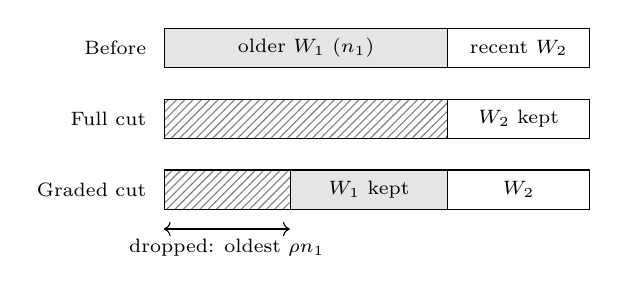
\begin{tikzpicture}[
  seg/.style={draw, minimum height=5mm, inner sep=0pt, font=\scriptsize},
  lab/.style={font=\scriptsize, anchor=east}
]
\def\a{3.6} \def\b{1.8} \def\d{1.6} \pgfmathsetmacro{\r}{\a-\d}
\node[lab] at (0,0) {Before};
\node[seg, minimum width=\a cm, fill=gray!20, anchor=west] (a1) at (0.1,0) {older $W_1$ ($n_1$)};
\node[seg, minimum width=\b cm, fill=white, anchor=west] (a2) at (\a+0.1,0) {recent $W_2$};
\node[lab] at (0,-0.9) {Full cut};
\node[seg, minimum width=\a cm, pattern=north east lines, pattern color=black!50, anchor=west] at (0.1,-0.9) {};
\node[seg, minimum width=\b cm, fill=white, anchor=west] at (\a+0.1,-0.9) {$W_2$ kept};
\node[lab] at (0,-1.8) {Graded cut};
\node[seg, minimum width=\d cm, pattern=north east lines, pattern color=black!50, anchor=west] at (0.1,-1.8) {};
\node[seg, minimum width=\r cm, fill=gray!20, anchor=west] at (\d+0.1,-1.8) {$W_1$ kept};
\node[seg, minimum width=\b cm, fill=white, anchor=west] at (\a+0.1,-1.8) {$W_2$};
\draw[<->, thin] (0.1,-2.3) -- node[font=\scriptsize, below] {dropped: oldest $\rho n_1$} (\d+0.1,-2.3);
\end{tikzpicture}
\caption{Window after a full cut (all of $W_1$ dropped, hatched) and after a graded cut (only the oldest part of $W_1$ dropped).}
\label{fig:cuts}
\end{figure}

The policy has three parts: a test at two confidence levels, a hold state that tracks persistence and a graded cut. Fig.~\ref{fig:states} shows the states and Algorithm~\ref{alg:policy} gives the full procedure.

\subsubsection{Two-level test}
We evaluate Eq.~\eqref{eq:eps} at a strict level $\delta_s$ and a relaxed level $\delta_w>\delta_s$, which gives two thresholds $\varepsilon_s>\varepsilon_w$ for each split. At a check we use the split with the largest normalized gap $|g|/\varepsilon_s$ and classify its evidence with the following rule, which is part of the proposed policy:
\begin{equation}
\text{evidence}=
\begin{cases}
\text{strong}, & |g|\ge\varepsilon_s,\\
\text{weak}, & \varepsilon_w\le|g|<\varepsilon_s,\\
\text{none}, & |g|<\varepsilon_w.
\end{cases}
\label{eq:zones}
\end{equation}
Strong evidence always causes a full cut and an alarm, exactly as in ADWIN-U.

\subsubsection{Hold state and persistence}
Weak evidence does not change the window. Instead the policy enters a hold state, raises a warning and stores the sign of $g$. A counter $c$ counts consecutive checks with weak evidence of the same sign. If the evidence drops to none or the sign of $g$ flips, the hold is released and $c$ is reset to zero. If $c$ reaches $k$, the change is treated as persistent and a graded cut is applied. A single unusual check therefore never cuts the window on its own.

\begin{figure}[!t]
\centering
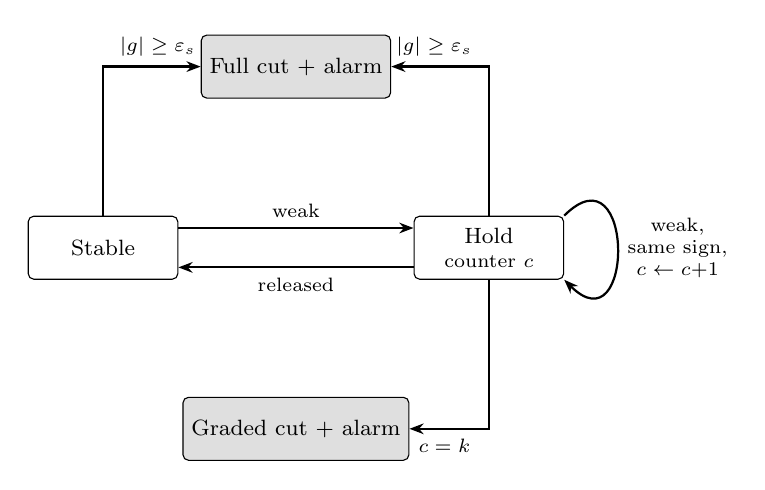
\begin{tikzpicture}[
  st/.style={draw, rounded corners=2pt, align=center, minimum height=8mm, minimum width=1.9cm, inner sep=3pt, font=\footnotesize, fill=white},
  ac/.style={draw, rounded corners=2pt, align=center, minimum height=8mm, inner sep=3pt, font=\footnotesize, fill=gray!25},
  arr/.style={-{Stealth[length=1.8mm]}, thick},
  lab/.style={font=\scriptsize, align=center}
]
\node[st] (stable) at (0,0) {Stable};
\node[st] (hold) at (4.9,0) {Hold\\[-1pt]{\scriptsize counter $c$}};
\node[ac] (full) at (2.45,2.3) {Full cut + alarm};
\node[ac] (grad) at (2.45,-2.3) {Graded cut + alarm};
\draw[arr] (stable.north) |- node[lab, pos=0.78, above] {$|g|\ge\varepsilon_s$} (full.west);
\draw[arr] (hold.north) |- node[lab, pos=0.78, above] {$|g|\ge\varepsilon_s$} (full.east);
\draw[arr] ([yshift=2.5mm]stable.east) -- node[lab, above] {weak} ([yshift=2.5mm]hold.west);
\draw[arr] ([yshift=-2.5mm]hold.west) -- node[lab, below] {released} ([yshift=-2.5mm]stable.east);
\draw[arr] (hold.south) |- node[lab, pos=0.78, below] {$c=k$} (grad.east);
\draw[arr] (hold.north east) .. controls +(0.9,0.9) and +(0.9,-0.9) .. node[lab, right, pos=0.5] {weak,\\same sign,\\$c\leftarrow c{+}1$} (hold.south east);
\end{tikzpicture}
\caption{States of the window-selection policy. A strong gap triggers an immediate full cut, while a weak gap starts a hold. The hold ends in a graded cut after $k$ consistent checks, or is released when the gap disappears or changes sign. After either cut the policy returns to Stable.}
\label{fig:states}
\end{figure}

\subsubsection{Graded cut}
A graded cut removes only the oldest part of $W_1$ (Fig.~\ref{fig:cuts}). We propose to set the share removed to
\begin{equation}
\rho=\min\!\Big(1,\frac{|g|}{\varepsilon_s}\Big),
\label{eq:rho}
\end{equation}
and the oldest $\lceil\rho\, n_1\rceil$ instances are dropped, rounded to whole buckets. Because a graded cut follows weak evidence, $\rho$ lies between $\varepsilon_w/\varepsilon_s$ and $1$, so a gap close to the strict threshold removes almost all of $W_1$ and a gap close to the relaxed threshold removes less. The reasoning behind this rule is that gradual or subtle drift can keep $|g|$ below $\varepsilon_s$ for a long time even after the old data no longer match the new data. ADWIN-U would keep the stale data until the gap finally crosses $\varepsilon_s$. The graded cut removes the oldest and most outdated part earlier while keeping the more recent part of $W_1$ in case the change is small. Both cuts raise an alarm, reset $c$ and, for the centroid signal, reset $c_i$.

\begin{algorithm}[htbp]
\caption{Window-selection policy (one check)}
\label{alg:policy}
\small
\begin{algorithmic}[1]
\Require window $W$, levels $\delta_s<\delta_w$, persistence $k$, state $(c,\sigma)$
\Ensure updated $W$, alarm flag
\State find the split $W_1\cdot W_2$ with the largest $|g|/\varepsilon_s$
\State compute $g$, $\varepsilon_s=\varepsilon(\delta_s)$, $\varepsilon_w=\varepsilon(\delta_w)$ by Eq.~\eqref{eq:eps}
\If{$|g|\ge\varepsilon_s$} \Comment{strong evidence}
  \State drop all of $W_1$; $c\gets0$; \Return alarm
\ElsIf{$|g|\ge\varepsilon_w$} \Comment{weak evidence}
  \If{$c=0$ \textbf{or} $\mathrm{sign}(g)=\sigma$}
    \State $c\gets c+1$; $\sigma\gets\mathrm{sign}(g)$; raise warning
  \Else
    \State $c\gets0$ \Comment{sign flipped: release}
  \EndIf
  \If{$c=k$}
    \State $\rho\gets\min(1,|g|/\varepsilon_s)$
    \State drop oldest $\lceil\rho n_1\rceil$ of $W_1$ (whole buckets)
    \State $c\gets0$; \Return alarm
  \EndIf
\Else
  \State $c\gets0$ \Comment{no evidence: release}
\EndIf
\State \Return no alarm
\end{algorithmic}
\end{algorithm}

\subsection{Properties and cost}

\subsubsection{ADWIN-U as a special case}
If $\delta_w=\delta_s$, the weak zone in Eq.~\eqref{eq:zones} is empty, the hold state is never entered and the policy behaves exactly like ADWIN-U. Any difference in results therefore comes from the hold state and the graded cut.

\subsubsection{Complexity}
Compared with ADWIN-U, the policy stores one counter and one sign and evaluates one extra threshold per split. Cuts remove whole buckets. We therefore expect the cost to stay at $O(\log|W|)$ time and memory per instance, and we measure it to confirm this. The centroid signal adds $O(D)$ time and memory per instance.

\subsubsection{False alarms}
The strict threshold keeps ADWIN's false-alarm guarantee, but a graded cut is triggered by the relaxed threshold together with persistence, so that guarantee no longer holds for it. We therefore measure false alarms on drift-free streams and calibrate all detectors to the same false-alarm rate before comparing them (Section~\ref{sec:protocol}).

%--------------------------------------------------------------------
\section{Experimental Design}
\label{sec:exp}

\subsection{Datasets and drift construction}
Table~\ref{tab:data} lists the datasets. On AG News \cite{zhang2015} we create drift by changing the mix of its four topic classes. Abrupt drift switches from one mix to another at a single point $t_d$. Gradual drift uses the sigmoid transition of Bifet et al.\ \cite{bifet2009}, which is also used in MOA \cite{bifet2010}. In this transition a document is drawn from the new mix with probability
\begin{equation}
p(t)=\frac{1}{1+e^{-4(t-t_d)/w}},
\end{equation}
where $w$ sets the width of the transition. Recurring drift returns to an earlier mix after a fixed interval. On 20 Newsgroups \cite{lang1995}, replacing groups with groups from a different macro-topic gives strong drift, and replacing groups with sibling groups from the same macro-topic gives subtle drift. Varying $w$ and the choice of groups lets us study drift type and magnitude separately. A drift-free version of each stream, with a fixed mix in random order, is used for calibration. As a real stream we use Amazon reviews \cite{ni2019} sorted by timestamp. Its drift points are unknown, so we use proxies: the alarm rate, the accuracy of a downstream classifier that is updated after each alarm under a fixed label budget and the alignment of alarms with known events. Together the datasets cover news, discussion posts and reviews, and range from known injected drift points to unknown real ones.

\begin{table}[!t]
\centering
\caption{Planned datasets.}
\label{tab:data}
\small
\begin{tabular}{>{\raggedright\arraybackslash}p{1.85cm}>{\raggedright\arraybackslash}p{3.6cm}>{\raggedright\arraybackslash}p{1.4cm}}
\toprule
Dataset & Role & Drift truth \\
\midrule
AG News & Abrupt, gradual, recurring drift by topic mix & Known \\
20 Newsgroups & Strong vs.\ subtle drift via macro-topics or sibling groups & Known \\
Amazon reviews & Real stream in time order & Unknown \\
\bottomrule
\end{tabular}
\end{table}

\subsection{Baselines}
We compare against ADWIN-U with single and multiple detectors \cite{assis2025}, plain ADWIN over a grid of $\delta$ values, a two-threshold warning and alarm variant of ADWIN, a KSWIN-style fixed-window test \cite{raab2020} and a D3-style discriminative detector \cite{gozuacik2019}. The $\delta$ grid and the warning variant check whether any gain comes only from tuning $\delta$ or from adding a warning zone rather than from the policy itself. All detectors receive the same signal, so differences come from the windowing.

\subsection{Evaluation metrics}
\label{sec:metrics}
An alarm counts as a true detection of drift $t_m$ if it is the first alarm in the interval $[t_m,t_m+\Delta_a]$, where $\Delta_a$ is an acceptance window. All other alarms are false alarms. For gradual drift, $t_m$ is the start of the transition. Over a stream of $N$ instances with $N_{\mathrm{FA}}$ false alarms and a set $\mathcal{D}\subseteq\mathcal{T}$ of detected drifts, we report the standard detection measures \cite{gama2014,bifet2017}
\begin{align}
\mathrm{MTD}&=\frac{1}{|\mathcal{D}|}\sum_{t_m\in\mathcal{D}}(\hat t_m-t_m), &
\mathrm{FA}_{1k}&=\frac{1000\,N_{\mathrm{FA}}}{N}, \nonumber\\
\mathrm{MDR}&=1-\frac{|\mathcal{D}|}{|\mathcal{T}|}, &&
\end{align}
which are the mean time to detection, false alarms per 1,000 instances and missed-drift rate. For efficiency we report the mean window length, per-instance latency, peak memory and throughput in documents per second. BAR \cite{assis2025} is reported as a secondary measure. Following \cite{lukats2025}, accuracy-based scores are not used as the main criterion because they can favor detectors that fire often.

\subsection{Experimental protocol}
\label{sec:protocol}
First, the main parameter of every detector ($\delta$, or $\delta_s$ for our policy) is tuned on the drift-free streams so that all detectors reach the same $\mathrm{FA}_{1k}$. Each detector is then run on several random orderings of every drifting stream. Detectors are ranked per stream and compared with the Friedman test followed by the Nemenyi post-hoc test \cite{demsar2006}. An ablation compares three variants: hold only (persistent weak evidence leads to a full cut), graded cut without persistence ($k=1$) and the full policy. A sensitivity study varies $\delta_w/\delta_s$ and $k$. Detector timings exclude encoding, since embeddings are cached.
%--------------------------------------------------------------------
%--------------------------------------------------------------------
\begin{thebibliography}{99}
\bibitem{gama2014} J.~Gama, I.~\v{Z}liobait\.{e}, A.~Bifet, M.~Pechenizkiy, and A.~Bouchachia, ``A survey on concept drift adaptation,'' \emph{ACM Comput.\ Surv.}, vol.~46, no.~4, art.~44, 2014, \doi{10.1145/2523813}.

\bibitem{lu2019} J.~Lu, A.~Liu, F.~Dong, F.~Gu, J.~Gama, and G.~Zhang, ``Learning under concept drift: A review,'' \emph{IEEE Trans.\ Knowl.\ Data Eng.}, vol.~31, no.~12, pp.~2346--2363, 2019, \doi{10.1109/TKDE.2018.2876857}.

\bibitem{garcia2024review} C.~M. Garcia, R.~Abilio, A.~L. Koerich, A.~S. Britto~Jr., and J.~P. Barddal, ``Concept drift adaptation in text stream mining settings: A systematic review,'' \emph{ACM Trans.\ Intell.\ Syst.\ Technol.}, vol.~16, no.~2, pp.~1--67, 2025, \doi{10.1145/3704922}.

\bibitem{hinder2024a} F.~Hinder, V.~Vaquet, and B.~Hammer, ``One or two things we know about concept drift---a survey on monitoring in evolving environments. Part A: Detecting concept drift,'' \emph{Front.\ Artif.\ Intell.}, vol.~7, art.~1330257, 2024, \doi{10.3389/frai.2024.1330257}.

\bibitem{lukats2025} D.~Lukats, O.~Zielinski, A.~Hahn, and F.~Stahl, ``A benchmark and survey of fully unsupervised concept drift detectors on real-world data streams,'' \emph{Int.\ J.\ Data Sci.\ Anal.}, vol.~19, pp.~1--31, 2025, \doi{10.1007/s41060-024-00620-y}.

\bibitem{bifet2007} A.~Bifet and R.~Gavald\`a, ``Learning from time-changing data with adaptive windowing,'' in \emph{Proc.\ SIAM Int.\ Conf.\ Data Mining}, 2007, pp.~443--448, \doi{10.1137/1.9781611972771.42}.

\bibitem{assis2025} D.~N. Assis and V.~M.~A. Souza, ``ADWIN-U: Adaptive windowing for unsupervised drift detection on data streams,'' \emph{Knowl.\ Inf.\ Syst.}, vol.~67, no.~11, pp.~10005--10034, 2025, \doi{10.1007/s10115-025-02523-1}.

\bibitem{webb2016} G.~I. Webb, R.~Hyde, H.~Cao, H.~L. Nguyen, and F.~Petitjean, ``Characterizing concept drift,'' \emph{Data Min.\ Knowl.\ Discov.}, vol.~30, no.~4, pp.~964--994, 2016, \doi{10.1007/s10618-015-0448-4}.

\bibitem{suarez2023} A.~L. Su\'arez-Cetrulo, D.~Quintana, and A.~Cervantes, ``A survey on machine learning for recurring concept drifting data streams,'' \emph{Expert Syst.\ Appl.}, vol.~213, art.~118934, 2023, \doi{10.1016/j.eswa.2022.118934}.

\bibitem{gama2004} J.~Gama, P.~Medas, G.~Castillo, and P.~Rodrigues, ``Learning with drift detection,'' in \emph{Advances in Artificial Intelligence (SBIA)}, LNAI vol.~3171, 2004, pp.~286--295, \doi{10.1007/978-3-540-28645-5_29}.

\bibitem{raab2020} C.~Raab, M.~Heusinger, and F.-M. Schleif, ``Reactive soft prototype computing for concept drift streams,'' \emph{Neurocomputing}, vol.~416, pp.~340--351, 2020, \doi{10.1016/j.neucom.2019.11.111}.

\bibitem{gozuacik2019} \"O.~G\"oz\"ua\c{c}\i k, A.~B\"uy\"uk\c{c}ak\i r, H.~Bonab, and F.~Can, ``Unsupervised concept drift detection with a discriminative classifier,'' in \emph{Proc.\ ACM Int.\ Conf.\ Inf.\ Knowl.\ Manag. (CIKM)}, 2019, pp.~2365--2368, \doi{10.1145/3357384.3358144}.

\bibitem{hoeffding1963} W.~Hoeffding, ``Probability inequalities for sums of bounded random variables,'' \emph{J.\ Amer.\ Statist.\ Assoc.}, vol.~58, no.~301, pp.~13--30, 1963, \doi{10.1080/01621459.1963.10500830}.

\bibitem{datar2002} M.~Datar, A.~Gionis, P.~Indyk, and R.~Motwani, ``Maintaining stream statistics over sliding windows,'' \emph{SIAM J.\ Comput.}, vol.~31, no.~6, pp.~1794--1813, 2002, \doi{10.1137/S0097539701398363}.

\bibitem{hinder2020} F.~Hinder, A.~Artelt, and B.~Hammer, ``Towards non-parametric drift detection via dynamic adapting window independence drift detection (DAWIDD),'' in \emph{Proc.\ Int.\ Conf.\ Mach.\ Learn.\ (ICML)}, PMLR vol.~119, 2020, pp.~4249--4259.

\bibitem{chen2024} J.~Chen, S.~Yang, T.~Gao, Y.~Ying, T.~Li, and P.~Li, ``Multi-type concept drift detection under a dual-layer variable sliding window in frequent pattern mining with cloud computing,'' \emph{J.\ Cloud Comput.}, vol.~13, art.~40, 2024, \doi{10.1186/s13677-023-00566-9}.

\bibitem{klinkenberg2000} R.~Klinkenberg and T.~Joachims, ``Detecting concept drift with support vector machines,'' in \emph{Proc.\ Int.\ Conf.\ Mach.\ Learn.\ (ICML)}, 2000, pp.~487--494.

\bibitem{kuncheva2009} L.~I. Kuncheva and I.~\v{Z}liobait\.{e}, ``On the window size for classification in changing environments,'' \emph{Intell.\ Data Anal.}, vol.~13, no.~6, pp.~861--872, 2009, \doi{10.3233/IDA-2009-0397}.

\bibitem{mehmood2024} H.~Mehmood, A.~Khalid, P.~Kostakos, E.~Gilman, and S.~Pirttikangas, ``A novel edge architecture and solution for detecting concept drift in smart environments,'' \emph{Future Gener.\ Comput.\ Syst.}, vol.~150, pp.~127--143, 2024, \doi{10.1016/j.future.2023.08.023}.

\bibitem{badar2023} M.~Badar, W.~Nejdl, and M.~Fisichella, ``FAC-fed: Federated adaptation for fairness and concept drift aware stream classification,'' \emph{Mach.\ Learn.}, vol.~112, pp.~2761--2786, 2023, \doi{10.1007/s10994-023-06360-7}.

\bibitem{hu2024} L.~Hu, W.~Li, Y.~Lu, and C.~Hu, ``Scalable concept drift adaptation for stream data mining,'' \emph{Complex Intell.\ Syst.}, vol.~10, pp.~6725--6743, 2024, \doi{10.1007/s40747-024-01524-x}.

\bibitem{reimers2019} N.~Reimers and I.~Gurevych, ``Sentence-BERT: Sentence embeddings using Siamese BERT-networks,'' in \emph{Proc.\ EMNLP-IJCNLP}, 2019, pp.~3980--3990, \doi{10.18653/v1/D19-1410}.

\bibitem{wang2020} W.~Wang, F.~Wei, L.~Dong, H.~Bao, N.~Yang, and M.~Zhou, ``MiniLM: Deep self-attention distillation for task-agnostic compression of pre-trained transformers,'' in \emph{Advances in Neural Information Processing Systems}, vol.~33, 2020.

\bibitem{joanes1998} D.~N. Joanes and C.~A. Gill, ``Comparing measures of sample skewness and kurtosis,'' \emph{J.\ Roy.\ Statist.\ Soc.\ Ser.\ D (The Statistician)}, vol.~47, no.~1, pp.~183--189, 1998, \doi{10.2307/2988433}.

\bibitem{salton1975} G.~Salton, A.~Wong, and C.~S. Yang, ``A vector space model for automatic indexing,'' \emph{Commun.\ ACM}, vol.~18, no.~11, pp.~613--620, 1975, \doi{10.1145/361219.361220}.

\bibitem{zhang2015} X.~Zhang, J.~Zhao, and Y.~LeCun, ``Character-level convolutional networks for text classification,'' in \emph{Advances in Neural Information Processing Systems}, vol.~28, 2015.

\bibitem{lang1995} K.~Lang, ``NewsWeeder: Learning to filter netnews,'' in \emph{Proc.\ Int.\ Conf.\ Mach.\ Learn.\ (ICML)}, 1995, pp.~331--339, \doi{10.1016/B978-1-55860-377-6.50048-7}.

\bibitem{ni2019} J.~Ni, J.~Li, and J.~McAuley, ``Justifying recommendations using distantly-labeled reviews and fine-grained aspects,'' in \emph{Proc.\ EMNLP-IJCNLP}, 2019, pp.~188--197, \doi{10.18653/v1/D19-1018}.

\bibitem{bifet2009} A.~Bifet, G.~Holmes, B.~Pfahringer, R.~Kirkby, and R.~Gavald\`a, ``New ensemble methods for evolving data streams,'' in \emph{Proc.\ ACM SIGKDD Int.\ Conf.\ Knowl.\ Discov.\ Data Mining}, 2009, pp.~139--148, \doi{10.1145/1557019.1557041}.

\bibitem{bifet2010} A.~Bifet, G.~Holmes, R.~Kirkby, and B.~Pfahringer, ``MOA: Massive online analysis,'' \emph{J.\ Mach.\ Learn.\ Res.}, vol.~11, pp.~1601--1604, 2010.

\bibitem{bifet2017} A.~Bifet, ``Classifier concept drift detection and the illusion of progress,'' in \emph{Artificial Intelligence and Soft Computing (ICAISC)}, LNCS, Springer, 2017, pp.~715--725, \doi{10.1007/978-3-319-59060-8_64}.

\bibitem{demsar2006} J.~Dem\v{s}ar, ``Statistical comparisons of classifiers over multiple data sets,'' \emph{J.\ Mach.\ Learn.\ Res.}, vol.~7, pp.~1--30, 2006.
\end{thebibliography}

\end{document}
